\documentclass{article}

\usepackage[margin=1in]{geometry}
\usepackage{listings}
\usepackage{color}
\usepackage{graphicx}
\usepackage{float}

\title{Lab 4: Analog to Digital Conversion and Display}
\date{October 24, 2017}
\author{Matthew Friedman 861151348\\Souradeep Bhattacharya 861105938\\EE128 Section: 021}

\definecolor{dkgreen}{rgb}{0,0.6,0}
\definecolor{gray}{rgb}{0.5,0.5,0.5}
\definecolor{mauve}{rgb}{0.58,0,0.82}

\lstset{frame=tb,
	language=C,
	aboveskip=3mm,
	belowskip=3mm,
	showstringspaces=false,
	columns=flexible,
	basicstyle={\small\ttfamily},
	numbers=none,
	numberstyle=\tiny\color{gray},
	keywordstyle=\color{blue},
	commentstyle=\color{dkgreen},
	stringstyle=\color{mauve},
	breaklines=true,
	breakatwhitespace=true,
	tabsize=4
}

\begin{document}
	\maketitle
	\section*{Abstract}
	The objective of this lab is to become familiar with ADCs and 7-segment displays. We conducted the same experiment twice: once on an Arduino and once on the Dragonboard.
	\section*{Experimental System Specification}
	The system we are required to build will read the input from the ADC and then display the output on the 7 segment display (from 0.0 to 5.0).
	\section*{Block Diagram}
	\subsection*{Dragonboard Diagram}
		\begin{figure}[H]
		\centering
		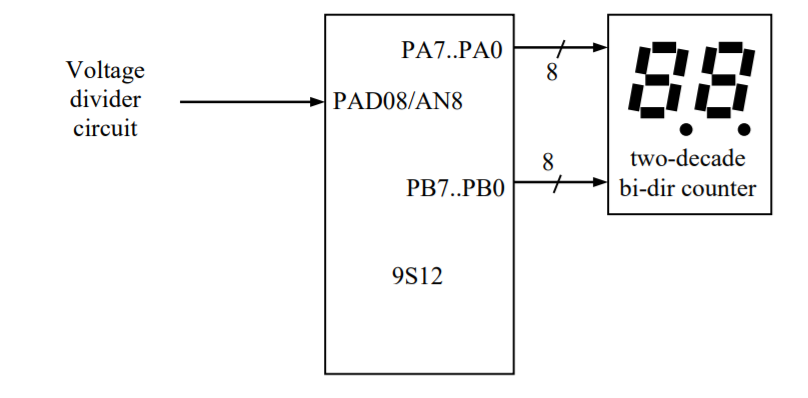
\includegraphics[width=1\textwidth]{Dragon_Block_Diagram}
	\end{figure}
	
	\subsection*{Arduino Diagram}
		\begin{figure}[H]
		\centering
		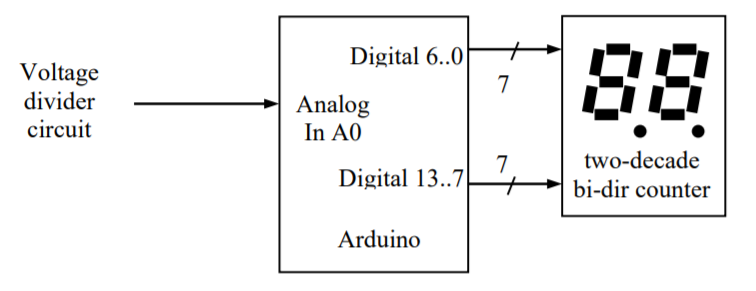
\includegraphics[width=1\textwidth]{Arduino_Block_Diagram}
	\end{figure}
	
	\section*{Detailed Schematic Diagram}
	\subsection*{Dragonboard Diagram}
		\begin{figure}[H]
		\centering
		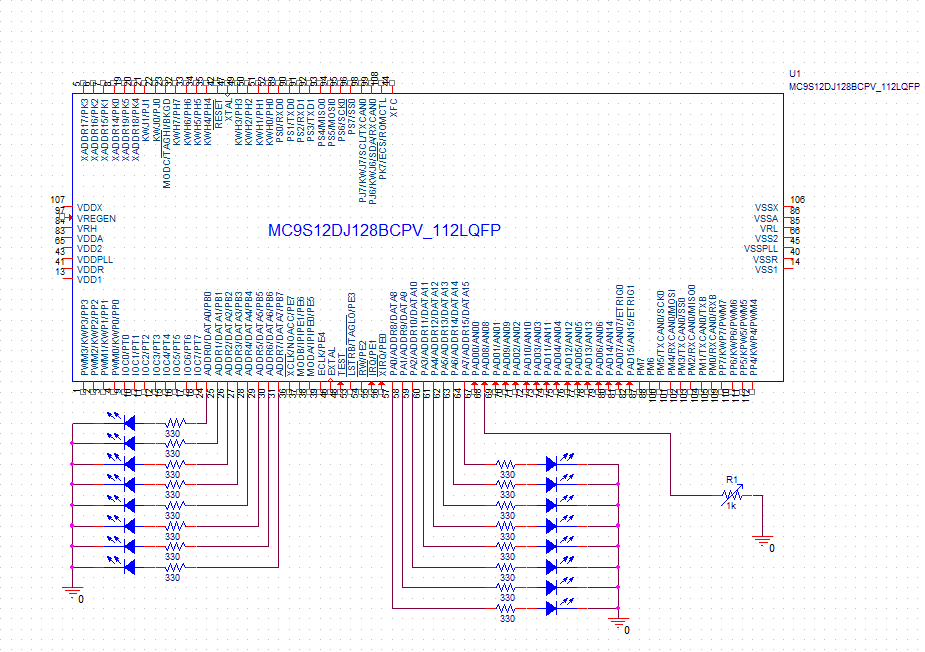
\includegraphics[width=1\textwidth]{Dragon_Diagram}
	\end{figure}
	
	\subsection*{Arduino Diagram}
		\begin{figure}[H]
		\centering
		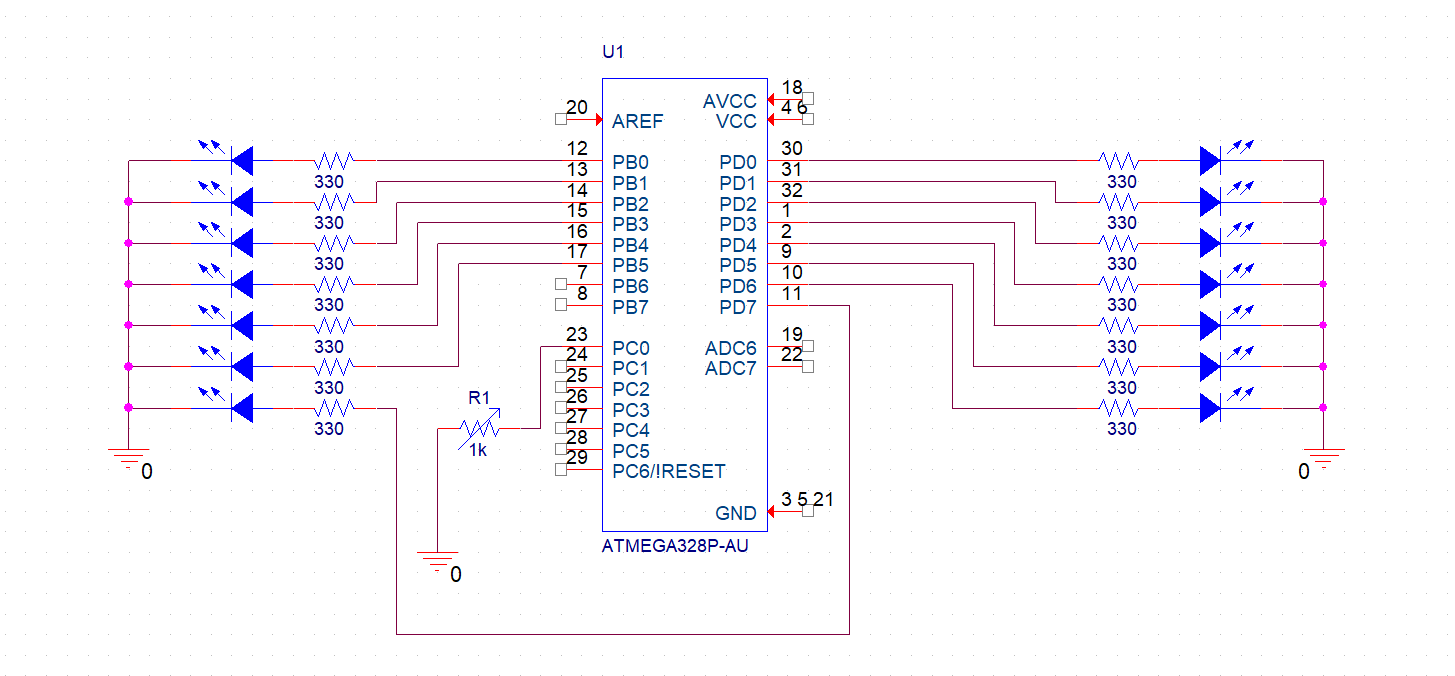
\includegraphics[width=1\textwidth]{Arduino_Diagram}
	\end{figure}
	
	\section*{High Level Description of the software}
	\par
	The pseudo code is as given:
	\begin{lstlisting}
	Configure Port A to be an 8-bit output port;
	Configure Port B to be an 8-bit output port;
	
	Initialize Port A;
	Initialize Port B;
	
	Turn on ADC;
	Wait at least 10 milliseconds for initialization;
	Configure ADC for 8/10-bit resolution;
	
	While (1)
	{	
		Wait for the A/D conversion completion flag in status register;
		Read the corresponding A/D result register;
		Send the result to the corresponding LED display;
	}
	\end{lstlisting}
	\section*{Program Listing}
	\subsection*{Dragonboard Program}
	\begin{lstlisting}
	#include <hidef.h>
	#include <mc9s12dg256.h>
	long i;
		
	float voltage = 0;
	int tens = 0;
	int ones = 0;
	unsigned char decoder[10] = {0x7E, 0x30, 0x6D, 0x79, 0x33, 0x5B, 0x5F, 0x70, 0x7F, 0x7B};
		
	void main(void) 
	{
		EnableInterrupts;
		
		DDRA = 0xFF;
		DDRB = 0xFF;
		
		ATD1CTL2 = 0xC0; // ATD power on, ATD fast flag clear bit
		for (i = 0; i < 150000; i++); // wait at least 20us for ATD stabilization
		ATD1CTL3 = 0x08; // 1 conversion
		ATD1CTL4 = 0xE0; // 0x60 for 10-bit, 0xE0 for 8-bit
		
		while (1) 
		{
			ATD1CTL5 = 0x84; // right-justified, AN8: voltage sensor
			while (!(ATD1STAT0 & 0x80)); // wait until conversion is done
		
			voltage =  ATD1DR0/255.0*5.0; //(/256.0 for 8 bit)
			tens = voltage;
			ones = (voltage*10) - (tens*10);
		
			//set port values
			PORTA = decoder[tens];
			PORTB = decoder[ones];
		
			for (i = 0; i < 50000; i++); // S/W Delay
		}
	}
		
	\end{lstlisting}
	\subsection*{Arduino Code}
	\begin{lstlisting}
	float voltage = 0.0;
	int tens = 0;
	int ones = 0;
	unsigned char decoder[10] = {0x7E, 0x30, 0x6D, 0x79, 0x33, 0x5B, 0x5F, 0x70, 0x7F, 0x7B};
		
	void setup() 
	{
		pinMode(A0, INPUT);
		pinMode(15, OUTPUT);
		DDRD = 0xFF;
		DDRB = 0xFF;
	}
		
	void loop() 
	{
		voltage = analogRead(A0)*5.0/1023.0;
		tens = voltage;
		ones = (voltage*10 - tens*10);
		
		PORTD = decoder[tens];
		PORTB = decoder[ones];
		digitalWrite(15, (decoder[ones] & 0x40));
		
		delay(50);
	}
	\end{lstlisting}
	\section*{Technical Problems}
	\paragraph*{Could get an ADC reading on Dragonboard}
	While we were sure that our voltage divider worked because we had checked the output via a multimeter, we could not get a reading on our Dragonboard ADC. Our solution was to set the control register 5 to 0x84 in the while loop.
	\section*{Answers to Questions}
	\subsection*{Prelab Questions}
	\begin{enumerate}
		\item The Dragonboard ADC uses Successive Approximation.
		\item The Arduino ADC uses Successive Approximation.
	\end{enumerate}
	\subsection*{Lab Questions}
	\begin{enumerate}
		\item At 8 bits our resolution is 19.5mV and at 10 bits our resolution is 4.9mV. However because our display only displays to the tenths place we can't use this extra resolution effectively.
	\end{enumerate}
	\section*{Conclusion}
	In this lab we learned how to use the ADC on the Dragonboard and on the Arduino. We gained an appreciation for the Arduino Foundation because they made this very easy. 
\end{document}